\documentclass[aspectratio=169]{beamer}

\usepackage[T1]{fontenc}
\usepackage[utf8]{inputenc}
\usepackage[ngerman]{babel}
\usepackage{lmodern}
\usepackage{hyperref}
\usepackage{graphicx}
\usepackage{xcolor}
\usepackage{booktabs}
\usepackage{array}

\graphicspath{{Screenshots/}{../Assets/UIs/}}

\usetheme{Madrid}
\usecolortheme{default}

\definecolor{dsgreen}{RGB}{43,102,74}
\definecolor{dsgold}{RGB}{193,149,45}
\definecolor{dsgray}{RGB}{48,48,48}

\setbeamercolor{title}{fg=white,bg=dsgreen}
\setbeamercolor{frametitle}{fg=white,bg=dsgreen}
\setbeamercolor{structure}{fg=dsgreen}
\setbeamercolor{block title}{fg=white,bg=dsgreen}
\setbeamercolor{block body}{fg=black,bg=black!3}
\setbeamercolor{palette primary}{fg=white,bg=dsgreen}
\setbeamercolor{palette secondary}{fg=white,bg=dsgray}
\setbeamercolor{palette tertiary}{fg=white,bg=dsgold}

\title{Dungeon Surge\\Abschlussprasentation}
\subtitle{2D Wave-Survival mit Bosskampfen, Upgrades und Level-Fortschritt}
\author{Bilgehan \and Fabian \and Selim Berk Tan}
\institute{Projektprasentation}
\date{30. Juni 2026}

\begin{document}

\begin{frame}
  \titlepage
\end{frame}

\begin{frame}{Kurzuberblick uber Team und Rollen}
  \begin{block}{Bilgehan}
    Skripte, Level 1 und Level 2 Design, Gegnerdesign, Player-Design, Player-Animationen und zentrale Gameplay-Logik.
  \end{block}

  \begin{block}{Fabian}
    Unterstutzung bei Scripts, Boss-Systemen, Level-up-Design, allgemeiner Gameplay-Hilfe, Upgrade-System und zwei Bosse.
  \end{block}

  \begin{block}{Selim Berk Tan}
    UI-Elemente wie Victory Screen und Endscreen, Soundeffekte, Audio-Integration und Game-End-Management.
  \end{block}
\end{frame}

\begin{frame}[shrink=3]{Finales Konzept und Designentscheidungen}
  \begin{columns}[T]
    \column{0.58\textwidth}
    \begin{itemize}
      \item Ziel: ein klar verstandliches 2D-Action-Spiel.
      \item Fokus auf kurze Core-Loop aus Kampf, XP und Upgrades.
      \item Zwei Level fur sichtbare Progression und Steigerung.
      \item Bosskampfe als klare Hohepunkte jeder Spielphase.
    \end{itemize}

    \column{0.42\textwidth}
    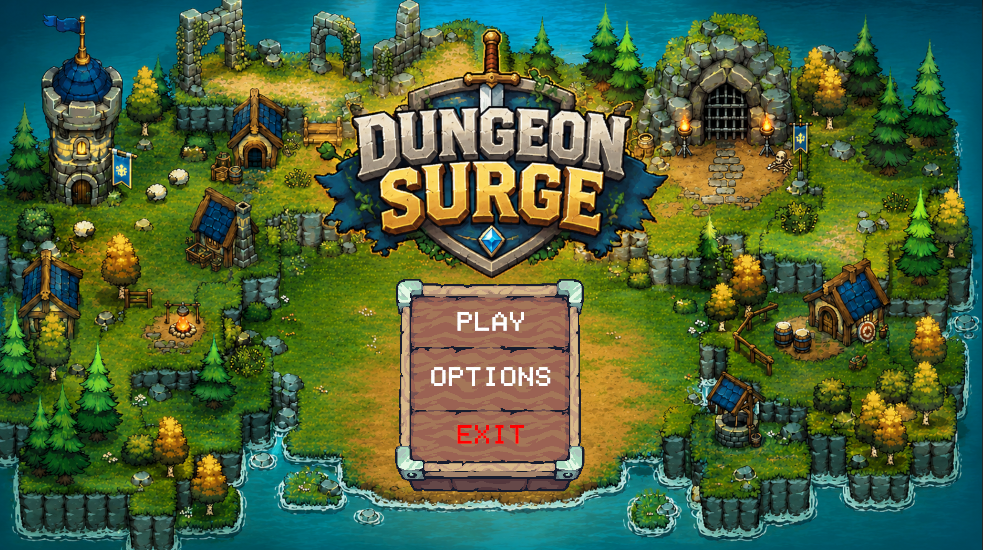
\includegraphics[width=\textwidth]{main-menu.png}
  \end{columns}
\end{frame}

\begin{frame}{Visuelle Designentscheidungen mit echten Assets}
  \begin{columns}[T]
    \column{0.5\textwidth}
    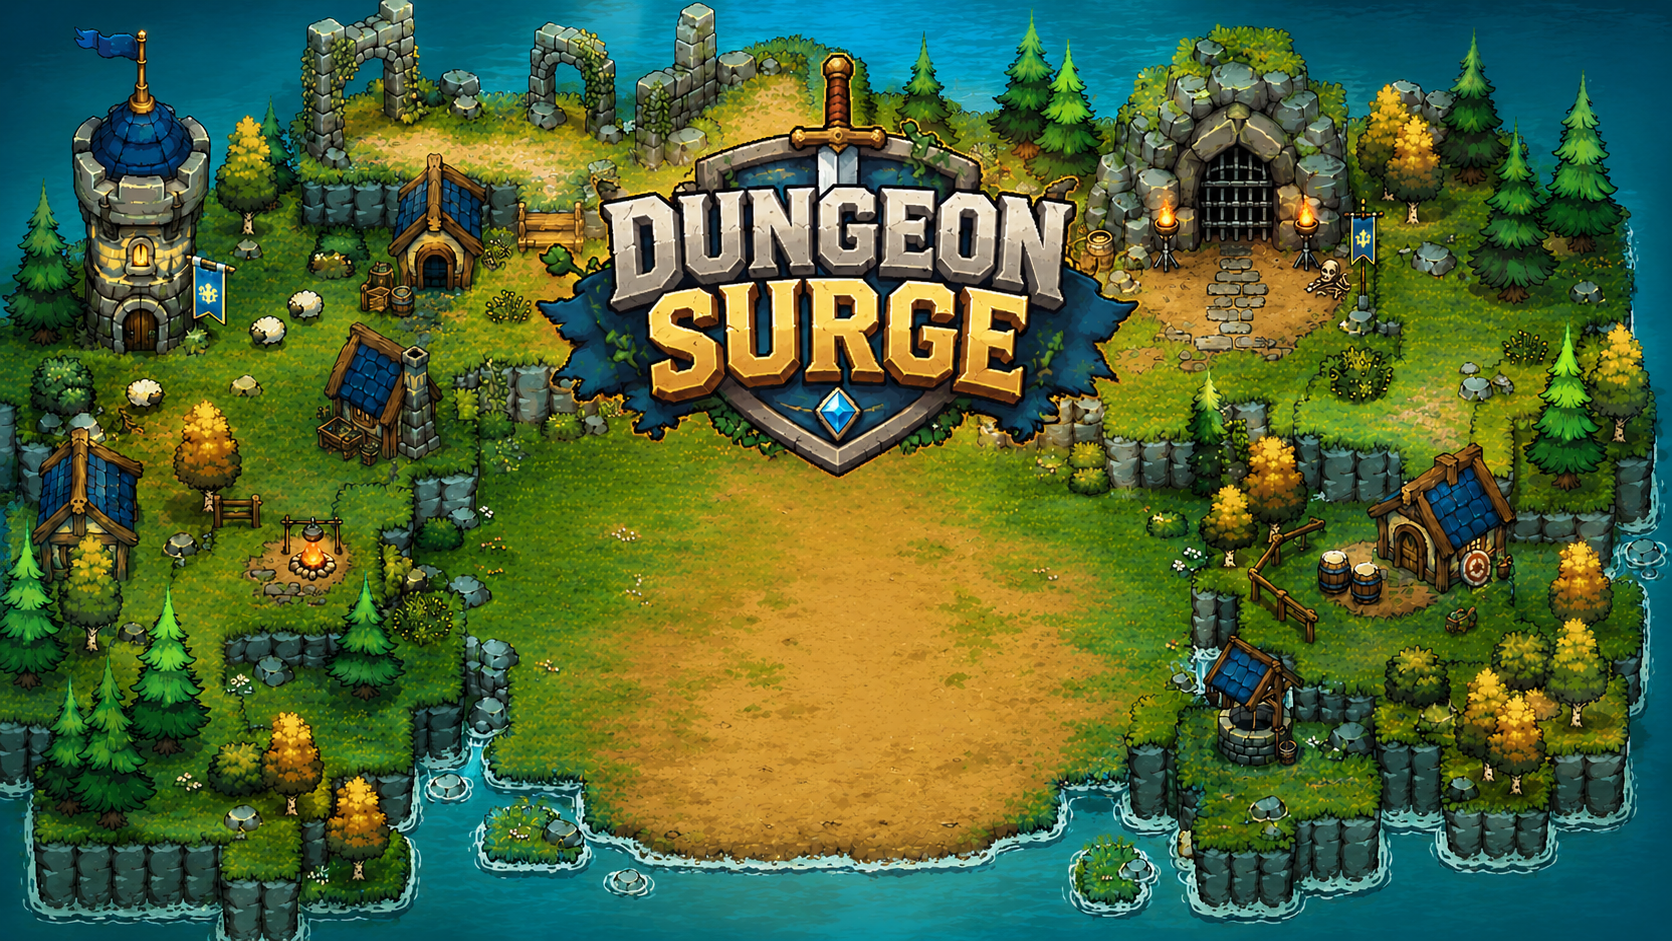
\includegraphics[width=\textwidth,height=0.28\textheight,keepaspectratio]{MainPage UI.png}\\[0.1cm]
    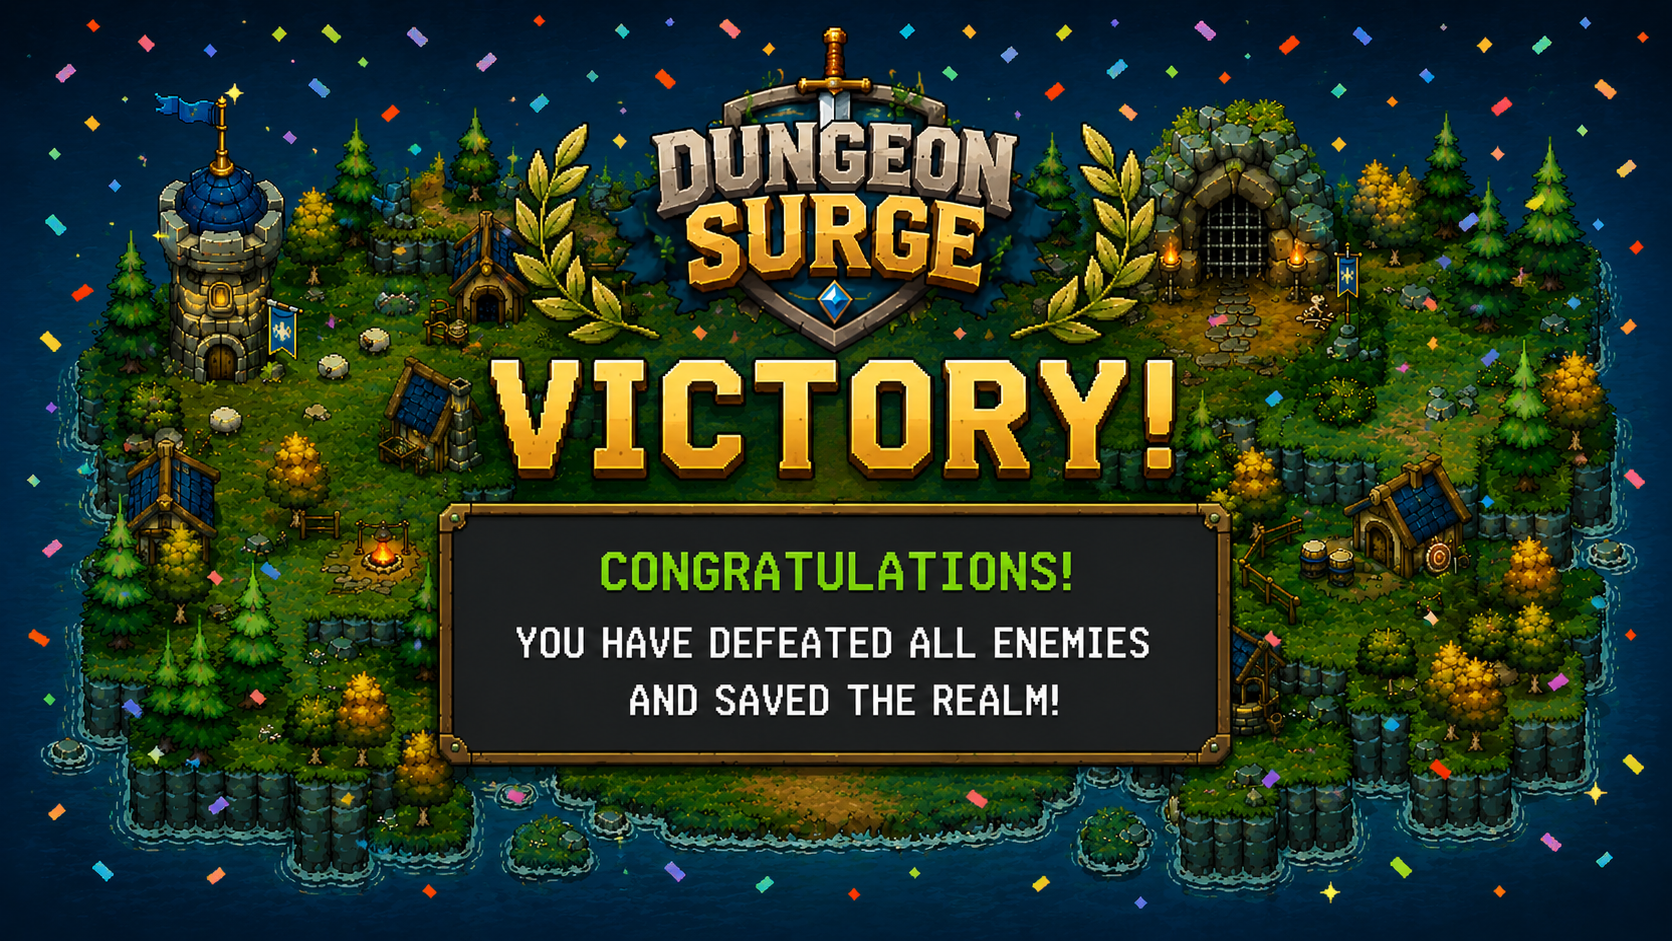
\includegraphics[width=\textwidth,height=0.18\textheight,keepaspectratio]{Victory.png}

    \column{0.5\textwidth}
    \small
    \begin{itemize}
      \item Einheitlicher Fantasy-Look fur Menu und HUD.
      \item Holz-, Stein- und Pergament-Optik passend zur Spielwelt.
      \item Große Buttons und klare Kontraste fur gute Lesbarkeit.
      \item Deutlicher Victory-Screen als starker Abschluss.
    \end{itemize}
  \end{columns}
\end{frame}

\begin{frame}{Tatsachlich verwendete Tools und Software}
  \begin{itemize}
    \item Engine: Unity mit 2D-Physik, Animation, Prefabs und Szenenverwaltung.
    \item Programmiersprache: C\# fur Gameplay-, UI-, Audio- und Progressionslogik.
    \item Projektstruktur: Szenen in \texttt{Assets/Scenes}, Skripte in \texttt{Assets/Scripts}, Gameplay-Prefabs in \texttt{Assets/Prefabs}.
    \item UI-Assets: vorhandene Screens fur Main Menu, Options, Level-Screens und Victory-Screens in \texttt{Assets/UIs}.
    \item Audio-Assets: Boss-Spawn, Boss-Fight, Treffer-, Gold-, Schwert- und weitere Sounds in \texttt{Assets/Audio}.
  \end{itemize}
\end{frame}

\begin{frame}{Projektaufbau im Code}
  \begin{columns}[T]
    \column{0.5\textwidth}
    \begin{block}{Szenen}
      \begin{itemize}
        \item MainMenu
        \item Level1
        \item Level2
      \end{itemize}
    \end{block}

    \begin{block}{Wichtige Prefabs}
      \begin{itemize}
        \item Pawn
        \item Lancer
        \item Boss\_GoblinKing
        \item Boss\_VampireBat
        \item Gold
        \item BossRockProjectile
      \end{itemize}
    \end{block}

    \column{0.5\textwidth}
    \begin{block}{Zentrale Skripte}
      \begin{itemize}
        \item WaveManager
        \item LevelManager
        \item UpgradeSelectionManager
        \item BossManager / BossHealth / BossController
        \item AudioManager
        \item LevelEndManager / VictoryManager
      \end{itemize}
    \end{block}
  \end{columns}
\end{frame}

\begin{frame}{Gameplay, Features und Mechaniken}
  \begin{columns}[T]
    \column{0.56\textwidth}
    \small
    \begin{itemize}
      \item Nahkampf, Bewegung und Sammeln bilden die Core-Loop des Spiels.
      \item Gold wird direkt in XP und Level-Fortschritt umgewandelt.
      \item Bei jedem Level-Up wahlt der Spieler eines von drei Upgrades.
      \item Upgrades verbessern Schaden, Leben, Tempo, Defense oder Regeneration.
    \end{itemize}

    \column{0.44\textwidth}
    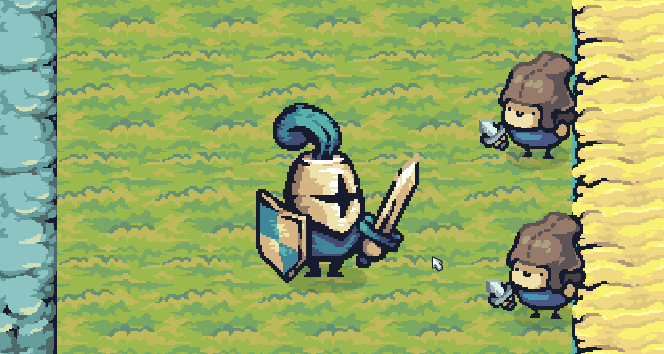
\includegraphics[width=\textwidth,height=0.55\textheight,keepaspectratio]{champion-closeup.png}
  \end{columns}
\end{frame}

\begin{frame}{Level 1 und Level 2 im Vergleich}
  \begin{columns}[T]
    \column{0.5\textwidth}
    \centering
    \textbf{Level 1}\\[0.2cm]
    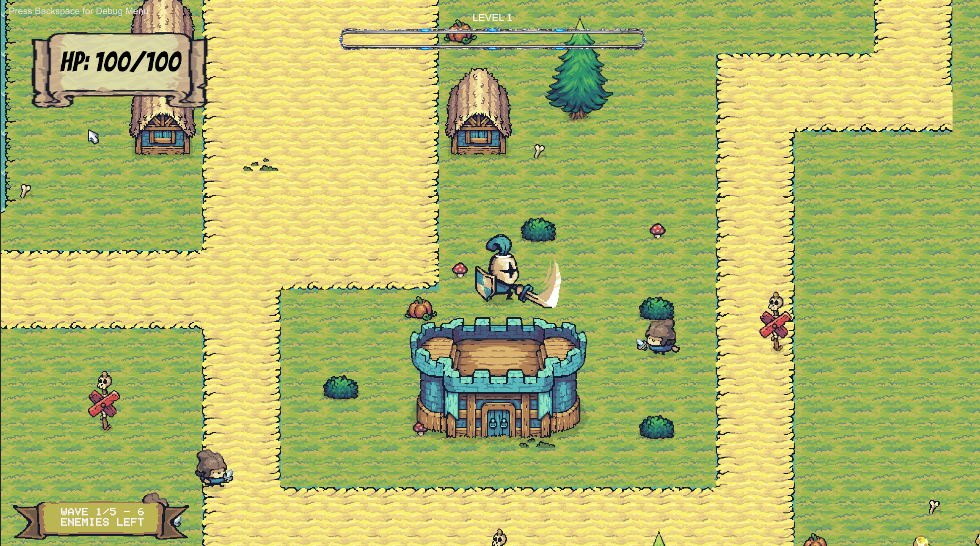
\includegraphics[width=\textwidth,height=0.31\textheight,keepaspectratio]{in-game-screen.png}\\[0.1cm]
    \scriptsize
    Grune Karte, offener Einstieg, fruhe Wellen und ein lesbarer Start in die Core-Loop.

    \column{0.5\textwidth}
    \centering
    \textbf{Level 2}\\[0.2cm]
    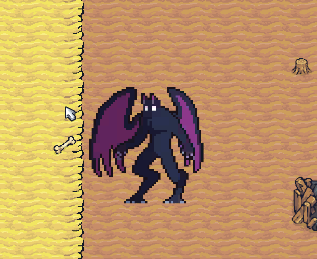
\includegraphics[width=\textwidth,height=0.31\textheight,keepaspectratio]{boss-2.png}\\[0.1cm]
    \scriptsize
    Anderes Farbklima, deutlich bedrohlichere Stimmung und Eskalation Richtung zweitem Bosskampf.
  \end{columns}

  \vspace{0.1cm}
  \small
  \begin{itemize}
    \item Der Unterschied zwischen beiden Levels ist absichtlich visuell klar: Level 1 wirkt klassisch-abenteuerlich, Level 2 harscher und boss-orientierter.
    \item So wird Fortschritt nicht nur uber Zahlen, sondern auch uber Umgebung, Ton und Kampfintensitat vermittelt.
  \end{itemize}
\end{frame}

\begin{frame}{Enemy-System und Wellenlogik}
  \begin{itemize}
    \item Gegner erscheinen in klar aufgebauten Wellen mit Countdown.
    \item Unterschiedliche Gegnertypen sorgen fur Abwechslung im Kampf.
    \item Erst wenn alle Gegner besiegt sind, startet die nachste Welle.
    \item Sichtbare Standardgegner sind Pawn und Lancer.
  \end{itemize}
\end{frame}

\begin{frame}{Boss-System und Bosskampfe}
  \begin{columns}[T]
    \column{0.52\textwidth}
    \begin{itemize}
      \item Bosskampfe werden mit Intro, Kamera-Fokus und Boss-Musik inszeniert.
      \item Beide Bosse haben mehrere Kampfphasen und eigene Angriffe.
      \item Goblin King setzt auf Nahkampf, Projektil und Charge.
      \item Vampire Bat ist der starkere Endboss mit aggressiverem Move-Set.
    \end{itemize}

    \column{0.48\textwidth}
    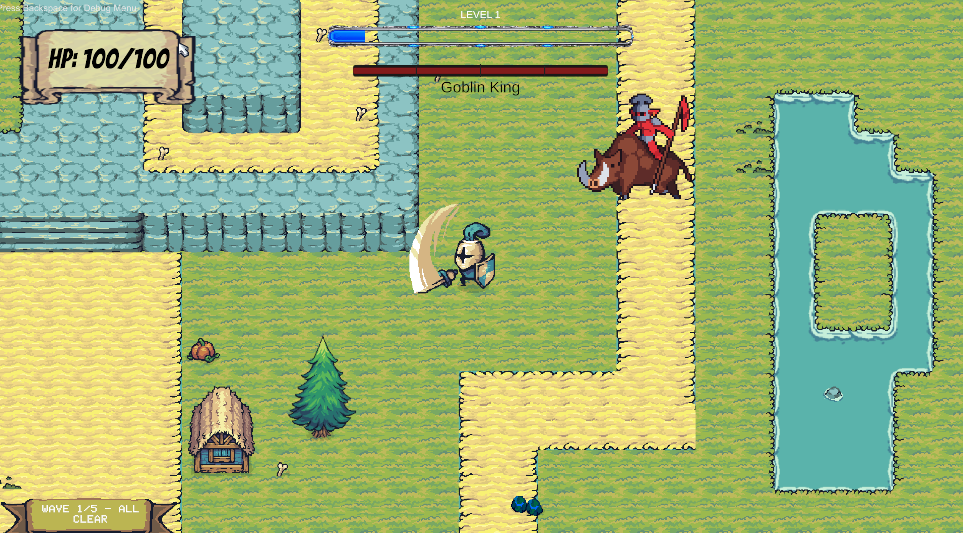
\includegraphics[width=\textwidth]{boss-fight.png}\\[0.15cm]
    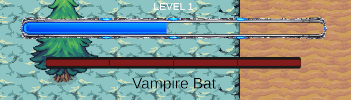
\includegraphics[width=\textwidth]{boss-level-bars.png}
  \end{columns}
\end{frame}

\begin{frame}{UI-, Audio- und Endgame-Flow}
  \begin{columns}[T]
    \column{0.56\textwidth}
    \begin{itemize}
      \item UI zeigt HP, XP, Wave-Status und Bossleiste klar und direkt.
      \item Musik und Soundeffekte unterstutzen Level-Up, Bosskampf und Victory.
      \item Nach Level 1 folgt der Ubergang in Level 2.
      \item Der Victory-Screen bildet den klaren Abschluss des Spiels.
    \end{itemize}

    \column{0.44\textwidth}
    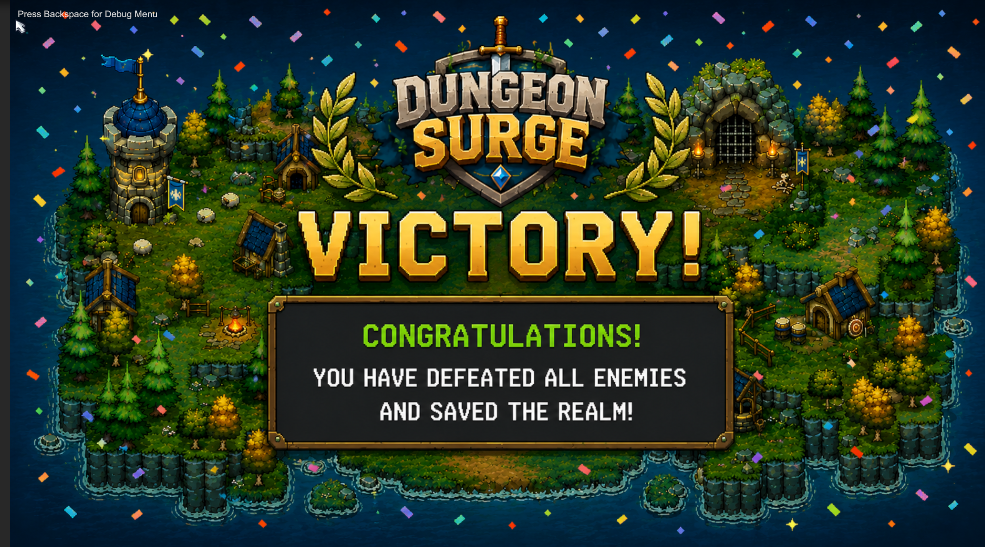
\includegraphics[width=\textwidth]{end-screen.png}
  \end{columns}
\end{frame}

\begin{frame}{Level-Fortschritt uber mehrere Szenen}
  \begin{itemize}
    \item \texttt{PlayerSessionData} speichert Level, XP, HP, Angriff, Speed, Defense und Regeneration zwischen Szenen.
    \item Dadurch bleibt die Progression von Level 1 nach Level 2 erhalten.
    \item Das unterstutzt die Spielidee, dass Level-Ups und Upgrades spurbare Auswirkungen auf den spateren Bosskampf haben.
    \item Technisch ist das eine einfache und robuste Losung ohne externes Save-System.
  \end{itemize}
\end{frame}



\begin{frame}[shrink=10]{Aufgetretene Probleme und Losungen}
  \small
  \begin{block}{1. Bosskampf-Inszenierung statt abruptem Spawn}
    Problem: Ein normaler Spawn wirkte technisch und unspektakular.\\
    Losung: \texttt{BossManager} kombiniert Kamera-Fokus, Overlay-Blinken, Spawn-SFX, Spawn-Delay und Boss-Musik zu einer kurzen Intro-Sequenz.
  \end{block}

  \begin{block}{2. Fortschritt uber zwei Level hinweg erhalten}
    Problem: Werte wie Level, XP und Upgrades durften beim Szenenwechsel nicht verloren gehen.\\
    Losung: \texttt{PlayerSessionData} speichert die relevanten Player-Werte vor dem Levelwechsel und stellt sie im nachsten Level wieder her.
  \end{block}

  \begin{block}{3. Lesbarkeit im Kampf trotz vieler Systeme}
    Problem: Wellen, XP, Boss-HP, Audio und Upgrade-Auswahl konnten schnell unubersichtlich werden.\\
    Losung: Trennung in Systeme wie \texttt{WaveUI}, \texttt{LevelUI}, \texttt{UpgradeSelectionManager} und \texttt{AudioManager}; zusatzlich pausiert die Upgrade-Auswahl das Spiel.
  \end{block}

  \begin{block}{4. Korrektes Wave-Ende}
    Problem: Eine Welle darf erst enden, wenn alles gespawnt und alles besiegt wurde.\\
    Losung: \texttt{WaveManager} verwaltet getrennt \texttt{enemiesToSpawn} und \texttt{enemiesAlive} und wartet auf beide Bedingungen.
  \end{block}
\end{frame}

\begin{frame}{Code-basierte Einordnung der Teamleistung}
  \begin{table}
    \scriptsize
    \begin{tabular}{p{0.23\textwidth} p{0.69\textwidth}}
      \toprule
      Person & Beitrag im Projekt \\
      \midrule
      Bilgehan & Kernskripte fur Spieler, Level, Wellen, Gegner, Session-Fortschritt sowie Level 1 und Level 2 als spielbare Struktur. \\
      Fabian & Unterstutzung bei Bosslogik, Upgrade-System, Level-up-Design und allgemeiner Gameplay-Feinabstimmung. \\
      Selim Berk Tan & UI-Finishing, Victory- und Endscreen, Soundeffekte und Abschlussfluss des Spiels. \\
      \bottomrule
    \end{tabular}
  \end{table}
\end{frame}



\begin{frame}{Fazit}
  \begin{itemize}
    \item Dungeon Surge besitzt eine klare Gameplay-Schleife aus Kampf, Ressourcen, XP, Upgrades und Boss-Fortschritt.
    \item Das Projekt kombiniert spielerische Lesbarkeit mit modularen Unity-Systemen fur Gegner, Bosse, UI und Audio.
    \item Besonders stark ist die Verbindung aus Level-Progression, Upgrade-System und Boss-Inszenierung uber zwei Level hinweg.
  \end{itemize}

  \vspace{0.5cm}
  \centering
  \Large Fragen?
\end{frame}

\end{document}